
%\documentstyle[epsf,twocolumn]{jarticle}       %LaTeX2e仕様
% \documentclass[twocolumn]{jarticle}     %pLaTeX2e仕様(platex.exeの場合)
\documentclass[onecolumn]{ujarticle}   %pLaTeX2e仕様(uplatex.exeの場合)
%%%%%%%%%%%%%%%%%%%%%%%%%%%%%%%%%%%%%%%%%%%%%%%%%%%%%%%%%%%%%%
%%
%%  基本バージョン
%%
%%%%%%%%%%%%%%%%%%%%%%%%%%%%%%%%%%%%%%%%%%%%%%%%%%%%%%%%%%%%%%%%
\setlength{\topmargin}{-45pt}
%\setlength{\oddsidemargin}{0cm}
\setlength{\oddsidemargin}{-7.5mm}
%\setlength{\evensidemargin}{0cm}
\setlength{\textheight}{24.1cm}
%setlength{\textheight}{25cm}
\setlength{\textwidth}{17.4cm}
%\setlength{\textwidth}{172mm}
\setlength{\columnsep}{11mm}

%\kanjiskip=.07zw plus.5pt minus.5pt


% 【節が変わるごとに (1.1)(1.2) … (2.1)(2.2) と数式番号をつけるとき】
%\makeatletter
%\renewcommand{\theequation}{%
%\thesection.\arabic{equation}} %\@addtoreset{equation}{section}
%\makeatother

%\renewcommand{\arraystretch}{0.95} 行間の設定
%%%%%%%%%%%%%%%%%%%%%%%%%%%%%%%%%%%%%%%%%%%%%%%%%%%%%%%%
%\usepackage{graphicx}   %pLaTeX2e仕様(\documentstyle ->\documentclass)
\usepackage[dvipdfmx]{graphicx}
\usepackage{subcaption}
\usepackage{multirow}
\usepackage{amsmath}
\usepackage{url}
\usepackage{ulem}
\usepackage{algorithm}
\usepackage{algorithmic}
\usepackage{listings} %,jlisting} %日本語のコメントアウトをする場合jlistingが必要
%ここからソースコードの表示に関する設定
\lstset{
  basicstyle={\ttfamily},
  identifierstyle={\small},
  commentstyle={\smallitshape},
  keywordstyle={\small\bfseries},
  ndkeywordstyle={\small},
  stringstyle={\small\ttfamily},
  frame={tb},
  breaklines=true,
  columns=[l]{fullflexible},
  numbers=left,
  xrightmargin=0zw,
  xleftmargin=3zw,
  numberstyle={\scriptsize},
  stepnumber=1,
  numbersep=1zw,
  lineskip=-0.5ex
}
\newcommand{\argmax}{\mathop{\rm arg~max}\limits}
\newcommand{\argmin}{\mathop{\rm arg~min}\limits}

%%%%%%%%%%%%%%%%%%%%%%%%%%%%%%%%%%%%%%%%%%%%%%%%%%%%%%%%
\begin{document}

	%bibtex用の設定
	%\bibliographystyle{ujarticle}

	% \twocolumn[
		\noindent
		\hspace{1em}
		2022 年 5 月 27 日
		ゼミ資料
		\hfill
		杉山 竜弥
		\vspace{2mm}

		\hrule
		\begin{center}
			{\Large \bf 進捗報告}
		\end{center}
		\hrule
		\vspace{9mm}
	% ]


\section{今週やったこと}
\begin{itemize}
  \item スケッチの動画化
  \item 類似度指標
\end{itemize}

\section{スケッチの動画化}
スケッチデータを gif にした.

(別データ参照)

また今回のパラメータは学習済みのものを使っているはずだが,おもったよりも再現性が低い.他の学習済みパラメータも試してみて,上手くいかなければ追加学習をするのがよいかもしれない.
  % \begin{figure}[h]
  %   \begin{center}
  %     \includegraphics[clip,width=120mm]{sketch.gif}
  %     \caption{gif}
  %     \label{fig:result1}
  %   \end{center}
  % \end{figure}

\section{類似度指標}
先行研究で用いられていた Structural Similarity (SSIM) は 2 つの画像間での類似指標であり,
一般に画質の劣化を評価するために利用される.
先行研究はこの類似度指標について議論されており,
変換前の生のスケッチについて,「描き順」と画像化した「最終状態」の 2 つを考慮した複雑な指標となっていた.

あまりに複雑なのでまずは,変換後の潜在変数についてコサイン類似度を使ってスケッチを比較した.
データセット内に含まれる 2 つのイラストを取り出し,エンコードした潜在変数 $z$ (= 128 次元)をコサイン類似度で評価した.結果を図 \ref{fig:result1}, \ref{fig:result2}, \ref{fig:result3}, \ref{fig:result4} に示す.

まずコサイン類似度自体を評価すると,同一のイラストでは 1 になり機能している可能性は高いが,その他の例ではかなり絶対値が小さくなった.まだ詳しくはわかっていないが次元の呪いが関係しているかもしれない.
先行研究は 1 ストロークごとに評価していたと認識しているので,複雑な形状だとそもそも難しいということも考えられる.

\section{tensorflow のバージョン問題}
メインの Sketch RNN のコードは,tensorflow==1.1.0 で実装されているが,
公式サポートも終了しておりドキュメントが存在しないため,
今後複雑な実装をすることが困難になることが予想される.
時間はかかるが v2 系で実装されたものなどに移行することも検討したい.

\section{今後の予定}
スケッチの類似度指標としてコサイン類似度は,いまのままでは全く機能しないわけではないが最適な指標でもないということが分かった.先行研究の指標を試したいが,時間がかかることが予想される.

今後の予定としては以下を考えている.
\begin{itemize}
  \item スケッチの分解の方法
  \item 先行研究の類似度指標の導入(時間がかかりそう)
\end{itemize}


\newpage

\begin{figure}[th]
  \begin{center}
    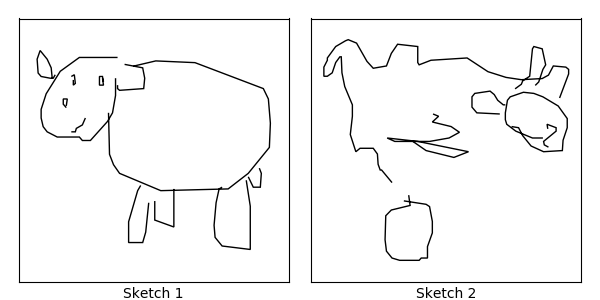
\includegraphics[clip,width=140mm]{compare.png}
    \caption{別々のイラスト -0.09293087}
    \label{fig:result1}
  \end{center}
\end{figure}

\begin{figure}[th]
  \begin{center}
    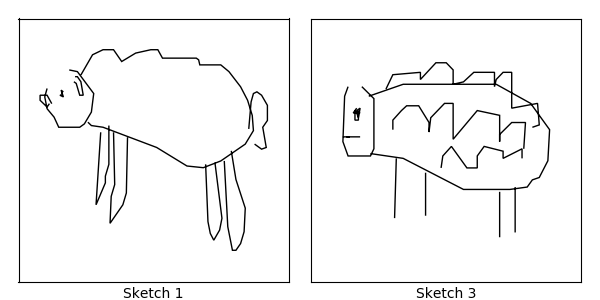
\includegraphics[clip,width=140mm]{compare2.png}
    \caption{別々のイラスト -0.021227952}
    \label{fig:result2}
  \end{center}
\end{figure}

\begin{figure}[th]
  \begin{center}
    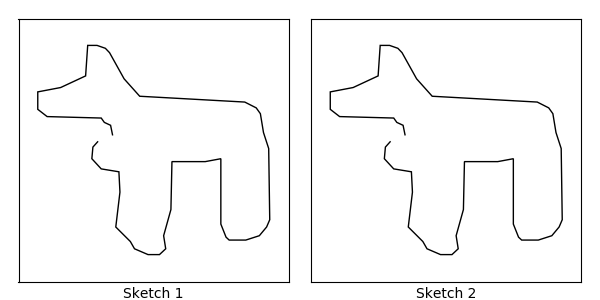
\includegraphics[clip,width=140mm]{compare3.png}
    \caption{同一のイラスト 1.0000001}
    \label{fig:result3}
  \end{center}
\end{figure}

\begin{figure}[th]
  \begin{center}
    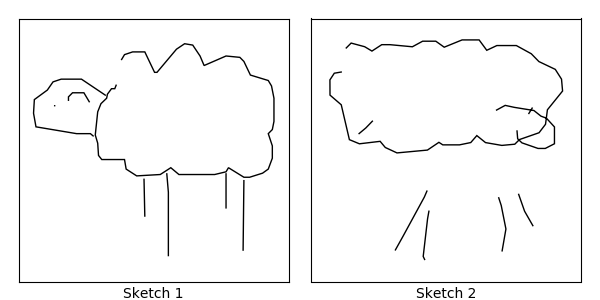
\includegraphics[clip,width=140mm]{compare4.png}
    \caption{再構築したイラスト 0.03555777}
    \label{fig:result4}
  \end{center}
\end{figure}






% 参考文献リスト
% \bibliographystyle{unsrt}
% \bibliography{ref}
\end{document}
